\documentclass[UKenglish]{beamer}


\usetheme{MathDept}
\usepackage{presentation}
\usepackage{style}


\day = 8
\month = 11
\year = 2017

\title{Join of hexagons and {Calabi--Yau} threefolds}
\subtitle{Public defence}
\author{Fredrik Meyer}


\begin{document}

\begin{frame}
\frametitle{Outline of the thesis}

\begin{itemize}
	\item Unsuccessful attempt to find new hyper-Kähler varieties.
	\item The topology of $C(\dP6)$.
	\item New Calabi--Yau varieties and potential mirror partners.
\end{itemize}

\end{frame}
\begin{frame}
\frametitle{\CY manifolds}

\begin{definition}%[\CY variety]
    A \alert{\CY variety} is a smooth projective scheme $X/\C$ of dimension~$3$ satisfying:
    \begin{itemize}
    	\item
	    $H^0(X,\OO_X)=H^3(X,\OO_X)=k$ and $h^1(X,\OO_X)=h^2(\OO_X)=0$.

	    \item
	    The canonical sheaf is trivial: $\omega_X \simeq \OO_X$. 
    \end{itemize}
\end{definition}

\unskip
\begin{columns}[onlytextwidth]
    \begin{column}{0.6\textwidth}
        \begin{itemize}
	        \item
	        Easiest invariants are the Euler characteristic and the Hodge numbers.

            \item
            We always have $\chi = 2(h^{11}-h^{12})$. 
        \end{itemize}
    \end{column}
\end{columns}

\only<1>
{
    \begin{textblock}{0.4}(0.58, 0.58)
        \[
            \arraycolsep = 1pt
            \def\arraystretch{0.5}
            \begin{array}[c]{ccccccc}
                &&& h^{00}                               \\  
                &&  h^{01} && h^{10}                     \\
                &   h^{02} && h^{11} && h^{20}           \\
                    h^{03} && h^{12} && h^{21} && h^{30} \\
                &   h^{13} && h^{22} && h^{31}           \\
                &&  h^{23} && h^{32}                     \\
                &&& h^{33} 
            \end{array}
        \]  
    \end{textblock}
}

\only<2>
{
    \begin{textblock}{0.4}(0.62, 0.62)
        \[
            \arraycolsep = 1.5pt
            \def\arraystretch{0.7}
            \begin{array}[c]{ccccccc}
                &&& 1                          \\
                &&  0 && 0                     \\
                &   0 && h^{11} && 0           \\
                    1 && h^{12} && h^{12} && 1 \\
                &   0 && h^{11} && 0           \\
                &&  0 && 0                     \\
                &&& 1 
            \end{array}
        \]
    \end{textblock}
}

\end{frame}
% This frame contains a lot of text
% with no highlighting or overlay effects

\begin{frame}
\frametitle{Hodge numbers}

The quintic $X = V(f) \subset \P^4$ is the canonical example of a \CY. It has Hodge numbers $h^{11}=1$ and $h^{12}=101$.

\begin{remark}[Heuristic]
    The number $h^{12}$ is the dimension of the ``space of parameters'' of $X$. The following heuristic will give us the correct Hodge number:
    \begin{itemize}
	    \item
	    The space of degree $5$ polynomials $H^0\big(\P^4, \OO_{\P^4}(5)\big)$ in $\P^4$ is $\binom{4 + 5}{5} = \binom{9}{4} = 126$-dimensional. Hence $\P\big(H^0\big(\P^4, \OO_{\P^4}(5)\big)\big) = \P^{125}$.

	    \item
	    This is not unique, but we can act by $\PGL(5)$ to identify isomorphic quintics. We have $\dim \PGL(5)=25-1=24$.

	    \item
	    In total: $125 - 24 = 101$, which is $h^{12}(X)$.
    \end{itemize}
\end{remark}

\end{frame}
\begin{frame}
\frametitle{Mirror symmetry}

\begin{itemize}
	\item \CY threefolds seem to ``always'' have ``mirror partners''.
	\item Mirror partner $X^\circ$ to $X$ have ``mirrored Hodge diamond''.
	\item Hence $\chi(X^\circ) = - \chi(X)$.
\end{itemize}

\unskip
\begin{columns}[onlytextwidth]
    \only<1->
    {
        \begin{column}{0.48\textwidth}
            \[
                \begin{array}[c]{ccccccc}
                    &&& X                    \\
                    \hline                   \\[-1.8ex]
                    &&& 1                    \\
                    &&  0 && 0               \\
                    &   0 && 1   && 0        \\
                        1 && 101 && 101 && 1 \\
                    &   0 && 1   && 0        \\
                    &&  0 && 0               \\
                    &&& 1
                \end{array}
            \]
        \end{column}
    }

    \only<2->
    {
        \begin{column}{0.48\textwidth}
            \[
                \begin{array}[c]{ccccccc}
                    &&& \phantom{^\circ}X^\circ \\
                    \hline                      \\[-1.8ex]
                    &&& 1                       \\  
                    &&  0 && 0                  \\
                    &   0 && 101 && 0           \\
                        1 && 1   && 1 && 1      \\
                    &   0 && 101 && 0           \\
                    &&  0 && 0                  \\
                    &&& 1
                \end{array}
            \]
        \end{column}
    }
\end{columns}


\end{frame}
\begin{frame}
\frametitle{The orbifold heuristic}

Sometimes the following method produces a mirror manifold of a Calabi--Yau $X$.

\begin{enumerate}
	\item \only<1>{Suppose $X$ has a natural degeneration $X_0$ with a finite automorphism group $G$.}
	\only<2->{
	\alert{The general quintic degenerates to the singular scheme $V(x_0x_1x_2x_3x_4)$.}} % Rød farge?

	\item \only<1-2>{Find a family $\pi: \mathscr X \to S$ on which $G$ act, and such that the general fiber $X_t$ have only isolated singularities.}
	\only<3->{
	\alert{
		The family defined by $f_t=x_0x_1x_2x_3x_4 +t \sum_{i=0}^4 x_i^5$ is $S_5$-invariant.
	}
	}

	\item \only<1-3>{There might be a finite subgroup $H$ of the big torus acting. A mirror candidate is then a crepant resolution of $X_t/H$.}
	\only<4->{
	\alert{
		There is an action of $H \stackrel \Delta = (\Z/5)^5/(\Z/5)$ on $X_t$. Crepant resolutions of $X_t/H$ exists, and is a mirror.
	}
	}
\end{enumerate}


\only<5->{
We can use \emph{Roan's formula} to compute the Euler characteristic.

\begin{theorem}[Roan's formula]
$$
\chi(\widetilde{X_t/H}) = \frac 1{|H|} \sum_{g,h \in H} \chi \left(X_t^g \cap X_t^h\right).
$$
\end{theorem}
}
\end{frame}
\begin{frame}
\frametitle{The cone over $\dP6$}

\begin{columns}
\column{0.5\textwidth}

\begin{itemize}
	\item Let $\dP6 \subset \P^6$ be an anticanonically embedded del Pezzo surface of degree $6$. Let $C(\dP6)$ be its affine cone in $\mathbb A^7$.

	\item The equations are 
	$$
\begin{vmatrix}
y & x_1 & x_2 \\
x_4 & y & x_3 \\
x_ 5 & x_6 & y
\end{vmatrix}
\leq 1
	$$

The origin is an isolated singularity.

\end{itemize}


\column{0.5\textwidth}

\begin{itemize}
	\item There are two smoothing components.
	\item They come from perturbations of differents form of writing the equation.
	\item Can also write the equations as:

	\begin{center}
	
	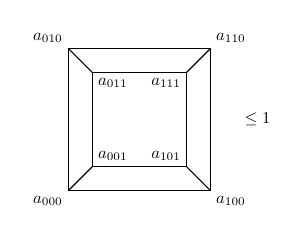
\begin{tikzpicture}[scale=0.6, every node/.style={scale=0.6}]
\draw (0,0) -- (3,0) -- (3,3) -- (0,3) -- cycle;
\draw (0.5,0.5) -- (2.5,0.5) -- (2.5,2.5) -- (0.5,2.5) -- cycle;
\draw (0,0) -- (0.5,0.5);
\draw (3,0) -- (2.5,0.5);
\draw (3,3) -- (2.5,2.5);
\draw (0,3) -- (0.5,2.5);
\node[below left] at (0,0) {$a_{000}$};
\node[below right] at (3,0) {$a_{100}$};
\node[above right] at (3,3) {$a_{110}$};
\node[above left] at (0,3) {$a_{010}$};

\node[above right] at (0.5,0.5) {$a_{001}$};
\node[above left] at (2.5,0.5) {$a_{101}$};
\node[below left] at (2.5,2.5) {$a_{111}$};
\node[below right] at (0.5,2.5) {$a_{011}$};

\node at (4, 1.5) {$\leq 1$};
\end{tikzpicture}
\end{center}
\end{itemize}


\end{columns}
\end{frame}


\end{document}